\documentclass{beamer}
\usetheme{Boadilla}

\usepackage{amsmath}
\usepackage{amsfonts}
\usepackage{hyperref}

\usepackage{amsmath}
\DeclareMathOperator*{\argmax}{arg\,max}
\DeclareMathOperator*{\argmin}{arg\,min}

\title{Dreaming to Distill: Data-free Knowledge Transfer via DeepInversion}
\author{Galina Boeva}
\institute{MIPT, 2024}


\begin{document}

\begin{frame}
    \titlepage
\end{frame}


\begin{frame}
    \tableofcontents
\end{frame}


\section{Motivation}
\begin{frame}{Motivation}
    \begin{block}{Main idea}
    Often having a huge predictive model, we would like to transfer knowledge from it to a more lightweight version that would be easy to build, for example, on a phone, but then the question arises of a training sample, we would like to transfer knowledge without data transfer.
    
    \end{block} 
    
\end{frame}

\begin{frame}{Background}
\textbf{Knowledge distillation}
\cite{breiman1996born} - Transfer of knowledge from one
model to another was first introduced by Breiman and
Shang when they learned a single decision tree to approximate the outputs of multiple decision trees. \cite{lopes2017data} - synthesize inputs based on pre-stored auxiliary layer-wise statistics of the teacher network.
\textbf{Image synthesis}
An alternative area of work without GAN in the field of security focuses on
the synthesis of images from a single CNN. \cite{fredrikson2015model} propose
an attack using model inversion to obtain class images from the network by gradient descent over the input data. \cite{mordvintsev2015inceptionism} has enabled
the “dreaming” of new object features onto natural images
given a single pretrained CNN.
\end{frame}

\section{DeepInversion}
\begin{frame}{Idea of method DeepInversion}
%\centering
\begin{figure}
        \centering
        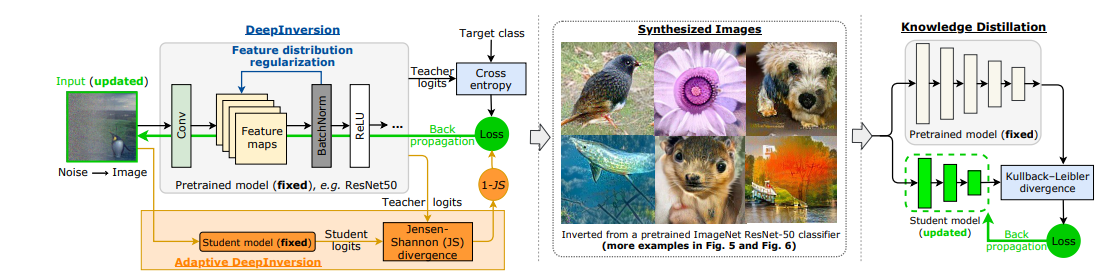
\includegraphics[scale=0.5]{images/distill_1.png}
        %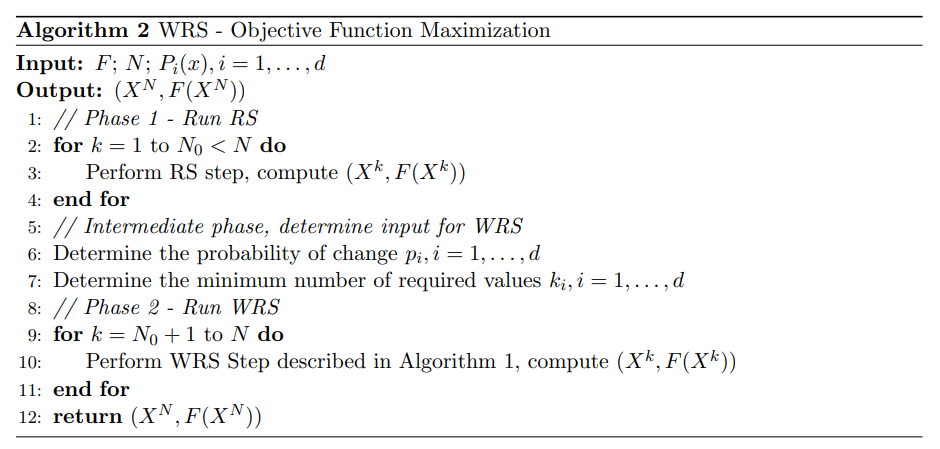
\includegraphics[scale=0.5]{images/wrs2.png}
        \caption{We introduce DeepInversion, a method that optimizes random noise into high-fidelity class-conditional images given just a pretrained CNN (teacher). Further, we introduce Adaptive DeepInversion, which utilizes both the teacher and application-dependent student network to improve image diversity. Using the synthesized images, we enable data-free pruning, introduce and address data-free knowledge transfer, and improve upon data-free continual learning.}
        \label{fig:enter-label}
    \end{figure}
\end{frame}

\begin{frame}{Method: Knowledge distillation\&DeepDream}
\begin{block}{Knowledge distillation}
Given a trained model $p_T$ and a dataset $\mathscr{X}$ , the parameters of the student model, $W_S$, can be learned by $\displaystyle\min_{\textbf{W}_S}\sum_{x \in \mathscr{X}} KL(p_T(x), p_S(x)),$ where $p_T(x) = p(x, \textbf{W}_T)$ and $p_S(x) = p(x, \textbf{W}_S)$ are the output distributions produced by the teacher and student model. 
\end{block}
\begin{block}{DeepDream}
DeepDream is also suitable for optimizing noise into images. Given a randomly initialized input and an arbitrary target label $y$, the image is synthesized by optimizing $\displaystyle\min_{\hat{x}} \mathscr{L}(\hat{x}, y) + \mathscr{R}(\hat{x})$, where $\mathscr{L}(\hat{x}, y)$ is a classification loss and
$\mathscr{R}(\hat{x})$ is an image regularization term. DeepDream uses an
image prior to steer $\hat{x}$ away from unrealistic images with no discernible visual information: $\mathscr{R}_{prior}(\hat{x}) = \alpha_{tv}\mathscr{R}_{TV}(\hat{x}) + \alpha_{l_2}\mathscr{R}_{l_2}(\hat{x})$, where $\mathscr{R}_{TV}$ and $\mathscr{R}_{l_2}$ penalize the total variance and $l_2$ norm
of $\hat{x}$, respectively, with scaling factors $\alpha_{tv}, \alpha_{l_2}$.
    
\end{block}
\end{frame}



\begin{frame}{DeepInversion}
\centering 
\begin{block}{DeepInversion}
    The feature distribution regularization term can be formulated as:
$$\mathscr{R}_{feature}(\hat{x}) = \displaystyle\sum{l} || \mu_{l}(\hat{x})-\mathbb{E}(\mu_{l}(x)|\mathscr{X})||_2 + \displaystyle\sum{l}||\sigma^2_l(\hat{x})-\mathbb{E}(\sigma^2_l(x)|\mathscr{X})||_2,$$
where $\mu_l(\hat{x})$ and $\sigma^2_l(\hat{x})$ are the batch-wise mean and variance
estimates of feature maps corresponding to the $l^{th}$ convolutional layer:
$$\mathbb{E}(\mu_{l}(x)|\mathscr{X}) \simeq BN_{l}(prunning\_mean), $$
$$ \mathbb{E}(\sigma^2_l(x)|\mathscr{X}) \simeq BN_{l}(prunning\_variance). $$
$\mathscr{R}(\cdot)$ can thus be expressed as
$$\mathscr{R}_{DI}(\hat{x})=\mathscr{R}_{prior}(\hat{x}) + \alpha_f \mathscr{R}_{feature}(\hat{x}) $$
\end{block}
\end{frame}

\begin{frame}{Adaptive DeepInversion}
\centering 

\begin{block}{Adaptive DeepInversion}
    Introduce an additional loss $\mathscr{R}_{compete}$ for image generation based on the Jensen-Shannon divergence that penalizes output distribution similarities,
$$\mathscr{R}_{compete}(\hat{x}) = 1 - JS(p_T(\hat{x}), p_S(\hat{x})). $$
$$\mathscr{R}_{ADI}(\hat{x}) = \mathscr{R}{DI}(\hat{x}) + \alpha_c \mathscr{R}{compete}(\hat{x})$$
\end{block}


\begin{figure}
        \centering
        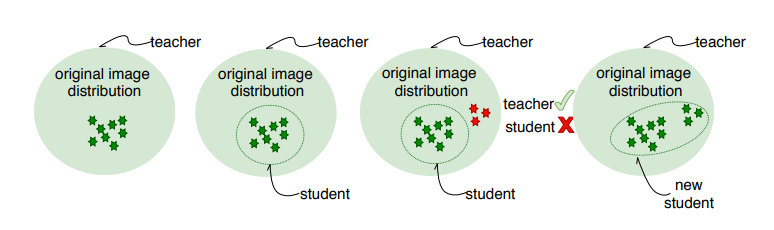
\includegraphics[scale=0.7]{images/distill_2.png}
        \caption{Illustration of the Adaptive DeepInversion competition
scheme to improve image diversity.}
    \end{figure}
 
\end{frame}


\section{Experiments of DI} 
\begin{frame}{Results on CIFAR-10}
    \begin{figure}
        \centering
        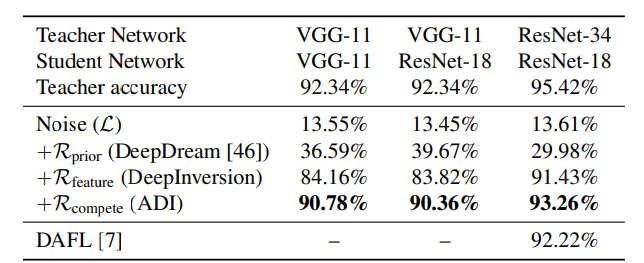
\includegraphics[scale=0.45]{images/distill_3.png}
        \caption{Data-free knowledge transfer to various students on
CIFAR-10.}
    \end{figure}
    \begin{figure}
        \centering
        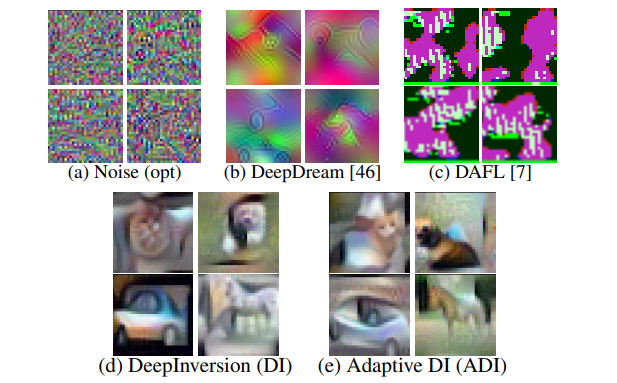
\includegraphics[scale=0.45]{images/distill_5.png}
        \caption{$32 \times 32$ images generated by inverting a ResNet-34
trained on CIFAR-10.}
        \label{fig:enter-label}
    \end{figure}
\end{frame}
\begin{frame}{Results on ImageNet}
    \begin{figure}
        \centering
        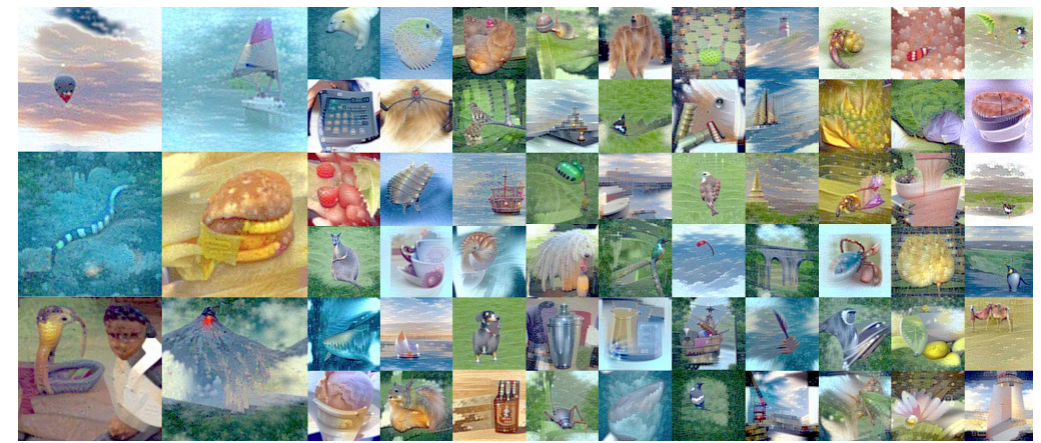
\includegraphics[scale=0.5]{images/distill_6.png}
        \caption{Class-conditional 224 ˆ 224 samples obtained by DeepInversion, given only a ResNet-50 classifier trained on ImageNet and no
additional information. Note that the images depict classes in contextually correct backgrounds, in realistic scenarios.}
        \label{fig:enter-label}
    \end{figure} 
\end{frame}

\begin{frame}{Results on ImageNet}
    \begin{figure}
        \centering
        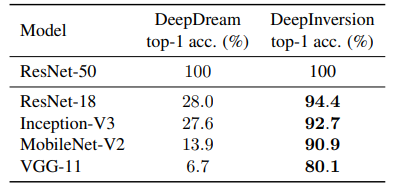
\includegraphics[scale=0.65]{images/distill_7.png}
        \caption{Classification accuracy of ResNet-50 synthesized images
by other ImageNet-trained CNNs.}
        \label{fig:enter-label}
    \end{figure}
    \begin{figure}
        \centering
        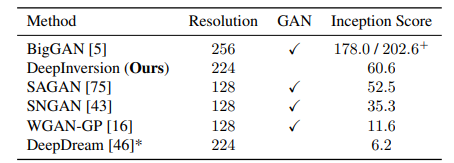
\includegraphics[scale=0.65]{images/distill11.png}
        \caption{Inception Score (IS) obtained by images synthesized by
various methods on ImageNet.}
        \label{fig:enter-label}
    \end{figure}
\end{frame}

\begin{frame}{Data-free Knowledge Transfer}
    \begin{figure}
        \centering
        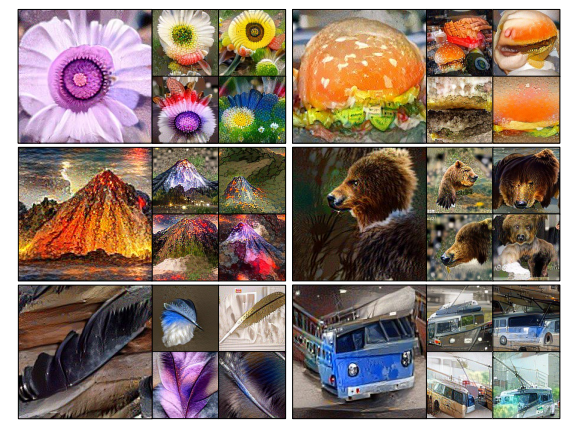
\includegraphics[scale=0.65]{images/distill8.png}
        \caption{Class-conditional $224 \times 224$ images obtained by DeepInversion given a ResNet50v1.5 classifier pretrained on ImageNet. Classes top to bottom: (left) daisy, volcano, quill, (right) cheeseburger, brown bear, trolleybus.}
        \label{fig:enter-label}
    \end{figure} 
\end{frame}

\begin{frame}{Data-free Pruning \& Data-free Continual Learning} 
    \begin{figure}[!tbp]
  \centering
  \begin{minipage}[b]{0.47\textwidth}
    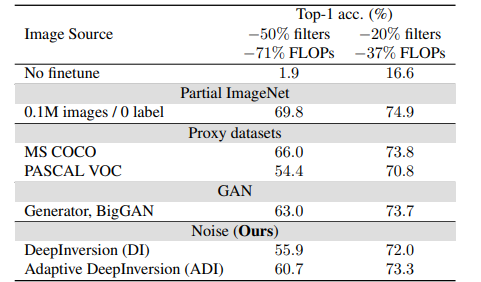
\includegraphics[width=\textwidth]{images/distill9.png}
    \caption{ImageNet ResNet-50 pruning comparison with prior work.}
  \end{minipage}
  \hfill
  \begin{minipage}[b]{0.5\textwidth}
    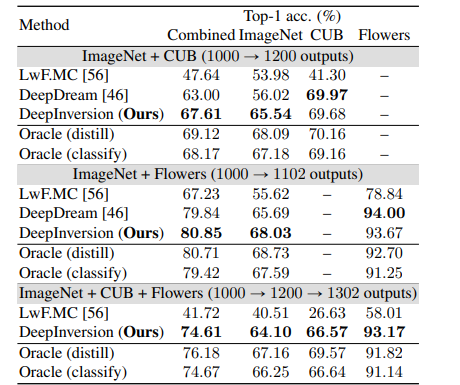
\includegraphics[width=\textwidth]{images/distill10.png}
    \caption{Continual learning results that extend the network output
space, adding new classes to ResNet-18.}
  \end{minipage}
\end{figure}
\end{frame}
 


\begin{frame}{Literature}
    \begin{enumerate}
        \item \textbf{Main article} \href{https://openaccess.thecvf.com/content_CVPR_2020/papers/Yin_Dreaming_to_Distill_Data-Free_Knowledge_Transfer_via_DeepInversion_CVPR_2020_paper.pdf}
        {Dreaming to Distill: Data-free Knowledge Transfer via DeepInversion}.
    \end{enumerate}
\end{frame}


\bibliographystyle{unsrt}
\bibliography{sample}
\end{document}